\pr (2b) Vyberte funkciu, ktorej definičný obor je znázornený na obrázku.
\begin{multicols}{2}
\noindent
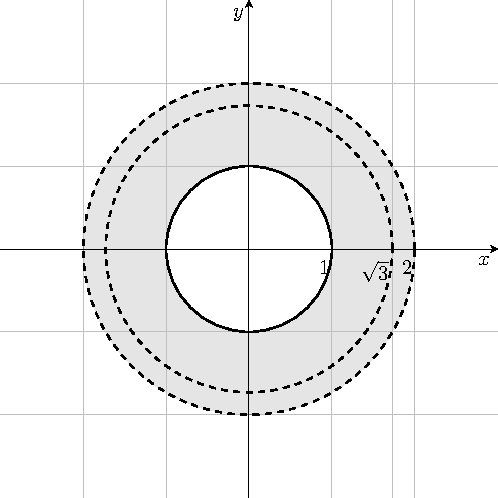
\includegraphics[width=6cm]{kruznica4.pdf}
\noindent
\begin{itemize}
\item[a)] $\displaystyle f(x,y)= \frac{\ln{(x^2+y^2-1)}}{\sqrt{4-x^2-y^2}}$
\item[b)] $\displaystyle f(x,y)= \frac{\sqrt{4-x^2-y^2}}{\ln(x^2+y^2-1)}$
\item[c)] $\displaystyle f(x,y)= \frac{\ln{(4-x^2-y^2)}}{\sqrt{x^2+y^2-1}}$
\item[d)] $\displaystyle f(x,y)= \frac{\sqrt{x^2+y^2-1}}{\ln{(4-x^2-y^2)}}$
\end{itemize}
\end{multicols}
